\documentclass[../main.tex]{subfiles}
\begin{document}
\clearpage
\setcounter{section}{0}% Сбрасываем счетчик в 0 (чтобы первое приложение было A)
\renewcommand{\thesection}{\Alph{section}}% Формат метки
\refstepcounter{section}
\section*{Приложение \Alph{section}.  Численный метод построения множеств достижимости при интегрально-квадратичных ограничениях на управление}% Заголовок с "Приложение A"
\label{app:A}% Метка с буквой (например, app:A)
\addcontentsline{toc}{section}{Приложение \Alph{section}. Численный метод построения множеств достижимости при интегрально-квадратичных ограничениях на управление}% Добавляем в оглавление
\renewcommand{\theequation}{\Alph{section}.\arabic{equation}}% Формат A.1 для формул
\setcounter{equation}{0}
  Построение множества достижимости управляемой динамической системы позволяет получить решение или хорошее начальное
  приближение для целого набора задач теории управления. 
  Множества достижимости играют важную роль при исследовании математических моделей и могут быть вспомогательным объектом для поиска управлений c обратной связью. 
  Существует множество методов построения оценок множеств достижимости. 
  Отметим здесь ряд работ \cite{Gornov2015, Gornov2017}, развивающих методы, основанные на заполнении множества достижимости набором точек, а также работы \cite{Lew2020, Lew2022}, в которых используется случайный выбор управлений и обеспечивается асимптотическая сходимость к выпуклой оболочке истинных множеств достижимости.
  В докладе рассматривается численный метод построения множеств достижимости нелинейных управляемых систем при интегрально-квадратичных ограничениях на управление. 
  Предлагаемый подход основывается на методе Монте-Карло с использованием случайного перебора управлений, разложенных по системе ортонормированных функций.
  
  На интервале времени $ t_0 \leqslant t \leqslant {T} $ рассмотрим нелинейную систему, аффинную по управлению
  \begin{gather}\label{a1:common_nonlinear}
  	\begin{gathered}
  		\dot{x}(t)=f\big(t, x(t), u(t)\big), \qquad x(t_0) = x_0.
  	\end{gathered}
  \end{gather}
  
  Здесь $ x \in \mathbb{R}^n $ ~--- вектор состояния, $ u \in \mathbb{R}^r $~--- управление,  $t_0$, $ {T} $ ~--- некоторые фиксированные положительные числа.
  
  Функция $ f: [t_0, {T}] \times  \mathbb{R}^n \times \mathbb{R}^r \rightarrow \mathbb{R}^{n} $ предполагается непрерывной по $(t,x,u)$ и обладающими непрерывными производными по $ x $ на  $ [t_0, {T}] \times \Omega \times \mathbb{R}^r $, где $\Omega$~--- некоторая область, $\Omega \subset \mathbb{R}^n$.  
  
  Всюду далее будем считать, что $x_0$ фиксирован и  $x_0 \in  \Omega $.
  Также будем предполагать, что существует такое $\overline{\mu} > 0 $, что все решения (траектории) $ x(t, u(\cdot)) $ системы \eqref{a1:common_nonlinear}, отвечающие управлениям $u(\cdot) \in B_{\mathbb{L}_2[t_0, {T}]}(0,\overline{\mu})$,  определены на интервале $ [t_0,{T}] $ и лежат в некотором выпуклом компакте $D \subset \Omega \subset \mathbb{R}^n$. 
  
  Через $\mathbb{L}_2[t_0, {T}]$ здесь обозначено пространство интегрируемых с квадратом функций на интервале $[t_0, {T}]$. 
  Под шаром $B_X(a,r)$ понимается замкнутый шар радиуса $r>0$ с центром в точке $a$ в линейном пространстве $X$ с нормой $\|\cdot\|_X$, $B_X(a, r) = \{x\in X: \|x-a\|_X \leqslant r \}$.
  
  В дальнейшем, управление $ u(\cdot) $ будем выбирать из шара $ B_{\mathbb{L}_2[t_0, {T}]}(0,\mu) $, где $ 0 < \mu < \overline{\mu} $, т.\,е.
  \begin{gather}\label{a1:constraints}
  	\int\limits_{t_0}^T u^{\top}(t) u(t) \ dt \leqslant \mu^2.
  \end{gather}
  
  {\sl Множеством достижимости } $ G(T,\mu) $ системы \eqref{a1:common_nonlinear} в пространстве состояний в момент времени $ T $ назовем множество всех концов траекторий $ x(T, u(\cdot)) \in \mathbb{R}^n $,  которые могут быть порождены управлениями $ u(\cdot) \in B_{\mathbb{L}_2}(0,\mu) =\left\lbrace u:\lVert u(\cdot)\rVert^2_{\mathbb{L}_2} \leqslant \mu^2\right\rbrace  $,
  \begin{gather*}
  	G(T,\mu)=\{x\in \mathbb{R}^n:\exists u(\cdot)\in B_{\mathbb{L}_2}(0,\mu),\; x=x(T,u(\cdot))\}.
  \end{gather*}
  
  Как и в других численных методах построения множеств достижимости, основанных на алгоритме Монте-Карло, идея обсуждаемого метода состоит в случайном переборе достаточно большого набора управлений $u_i(\cdot) \in U \subset B_{\mathbb{L}_2[t_0, {T}]}(0,\mu) $, каждое из которых удовлетворяет ограничению \eqref{a1:constraints}.
  Для каждого управления производится интегрирование системы \eqref{a1:common_nonlinear} и запоминается конечная точка полученной траектории $x_i(T, u_i(\cdot))$. 
  По определению, все такие точки лежат в множестве достижимости $G(T,\mu)$.
  
  Ключевым вопросом является конструирование множества управлений $U$.
  В случае геометрических ограничений, управления, которые ведут на границу, как правило, разрывны.
  Соответственно, для того, чтобы точнее построить границу множества достижимости, разумно строить множество перебираемых управлений именно из разрывных функций. 
  В случае же интегральных ограничений, на границу ведут, как правило, непрерывные ограничения. 
  В докладе предлагается заполнение этого множества управлениями вида 
  \begin{gather}
  	u_i(t) = C_i p (t),
  \end{gather}
  где $p(t) = \big(p_{0}(t),p_{1}(t),\dots,p_{k}(t)\big)$, $p: [t_0, {T}] \rightarrow \mathbb{R}^{k+1} $ --- вектор-функция, состоящая из ортонормированных скалярных функций в пространстве $\mathbb{L}_2[t_0, {T}]$, а $C_i \in \mathbb{R}^{r \times k+1}$ --- матрица коэффициентов. 
  
  Например, $p(t)$ для интервала $[0,1]$ можно составить из полиномов Лежандра:
  \begin{gather*}
  	p_0(t) = 1, \quad p_1(t) = 3.46t-1.73, \quad p_2(t) = 13.41t^2 - 13.41t + 2.24, \\ \quad 
  	p_3(t) = 52.92t^3 - 79.37t^2+31.75t -2.65, ...
  \end{gather*}
  
  Для того, чтобы такие управления, разложенные по системе ортонормированных функций, удовлетворяли ограничению \eqref{a1:constraints} оказывается достаточно, чтобы $\|C_i\| \leqslant \mu$, где $\|\cdot\| $ --- фробениусова норма матрицы.
  
  Ниже приведен псевдокод алгоритма построения множества достижимости системы \eqref{a1:common_nonlinear} с ограничениями \eqref{a1:constraints}.
  \RestyleAlgo{ruled}
  \begin{algorithm}[hbt!]
  	\SetKwFunction{Propagate}{Propagate}
  	\SetKwInOut{Parameters}{parameters}\SetKwInOut{Data}{data}\SetKwInOut{Output}{output}
  	\Parameters{Number of samples $N$, Degree of polynomial $k$}
  	\Data{Control resource $\mu$, Initial condition $x_0$, $t_0$, $T$}
  	\Output{$\{x_i\}_{i = 1}^{N}$}
  	$p(t) \gets $ Orthonormal polynomials in $\mathbb{L}_2[t,T]$ \;
  	\For{$i\leftarrow 0$ \KwTo $N$}{
  		$C \gets $ Random matrix from $B_{\mathbb{R}^{r \times k+1}}(0,\mu)$ \;
  		$u(t) \gets C p(t)$ \;
  		$x_i \gets $ \Propagate$\big(x_0, u(t), t_0, T\big)$\; }
  \end{algorithm}
  
  Полученное с помощью описанного алгоритма множество концов траекторий $\{x_i\}_{i = 1}^{N}$ при достаточно большом $N$ дает представление о форме и размерах множества достижимости и его проекций. 
  Итерации алгоритма не зависимы друг от друга, что позволяет вычислять концы траекторий $x_i$ параллельно. 
  Это, в свою очередь, позволяет увеличивать $N$, сохраняя время работы алгоритма в разумных пределах.
  
  \subsection{Простые примеры}
  На интервале времени $ 0 \leqslant t \leqslant 1$ рассмотрим линейную систему 
  \begin{gather*}
  	\begin{pmatrix} 
  		\dot{x}_1 \\
  		\dot{x}_2  
  	\end{pmatrix} = 
  	\begin{pmatrix}
  		0 & 1 \\
  		-2 & -3
  	\end{pmatrix}
  	\begin{pmatrix} 
  		x_1 \\
  		x_2  
  	\end{pmatrix} +
  	\begin{pmatrix} 1 \\ 0
  	\end{pmatrix} u
  \end{gather*}
  при ограничениях на управление 
  \begin{gather*}
  	\int\limits_0^1 u^2dt \leqslant 1.
  \end{gather*}
  \begin{figure}[ht!] 
  	\hspace{-2.5ex}
  	\begin{minipage}[b]{.49\linewidth} 
  		\small
  		\centering 
  		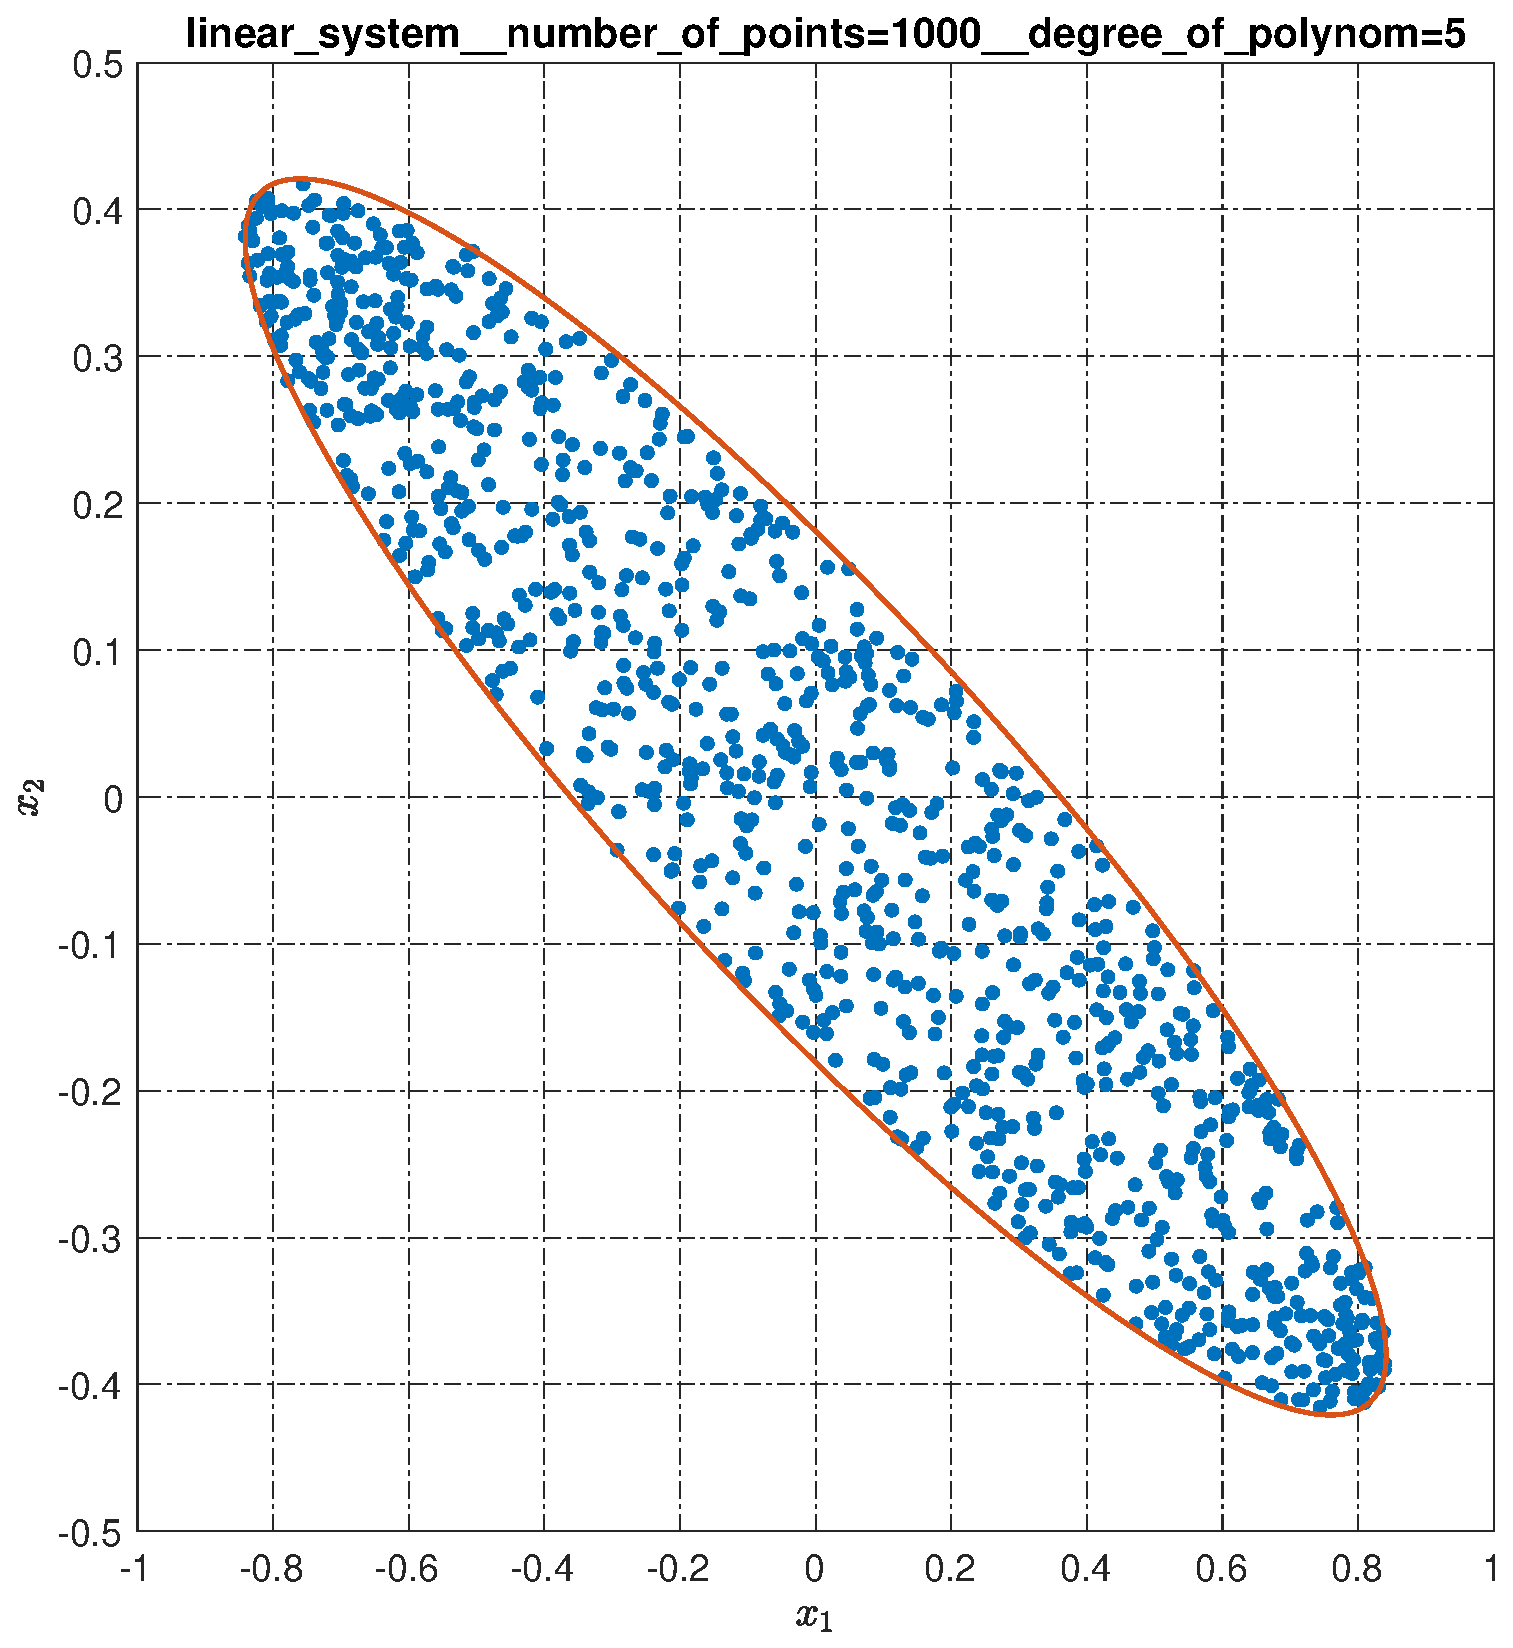
\includegraphics[width=\linewidth]{images/linear_system__number_of_points=1000__degree_of_polynom=5.eps}
  		%% This file was created by matlab2tikz.
%
%The latest updates can be retrieved from
%  http://www.mathworks.com/matlabcentral/fileexchange/22022-matlab2tikz-matlab2tikz
%where you can also make suggestions and rate matlab2tikz.
%
\begin{tikzpicture}
\node at (2.97,2.35) 
{
\includegraphics[width=0.985\linewidth]{images/OsipovI_u=0_x1-x2_1.eps}};
\pgfkeys{/pgf/number format/relative*={-3}}
\begin{axis}[%
width=0.761\linewidth,
height=0.6\linewidth,
at={(0\linewidth,0\linewidth)},
scale only axis,
xmin=0.009975,
xmax=0.01,
xlabel style={font=\color{white!15!black}},
xlabel={$ x_1 $},
ymin=-0.0006,
ymax=0.0006,
ylabel style={font=\color{white!15!black}},
ylabel={$ x_2 $},
xmajorgrids,
ymajorgrids,
grid style={dashed, opacity=0.7}
]
\end{axis}
\end{tikzpicture}%
%  		\subcaption{$ \overline{G}_{1,2}(\varepsilon) $ системы \eqref{unicycle0};}
%  		\label{fig:u=0_x1-x2} 
  	\end{minipage}
  	\hfill
  	\begin{minipage}[b]{.49\linewidth} 
  		\small
  		\centering
  		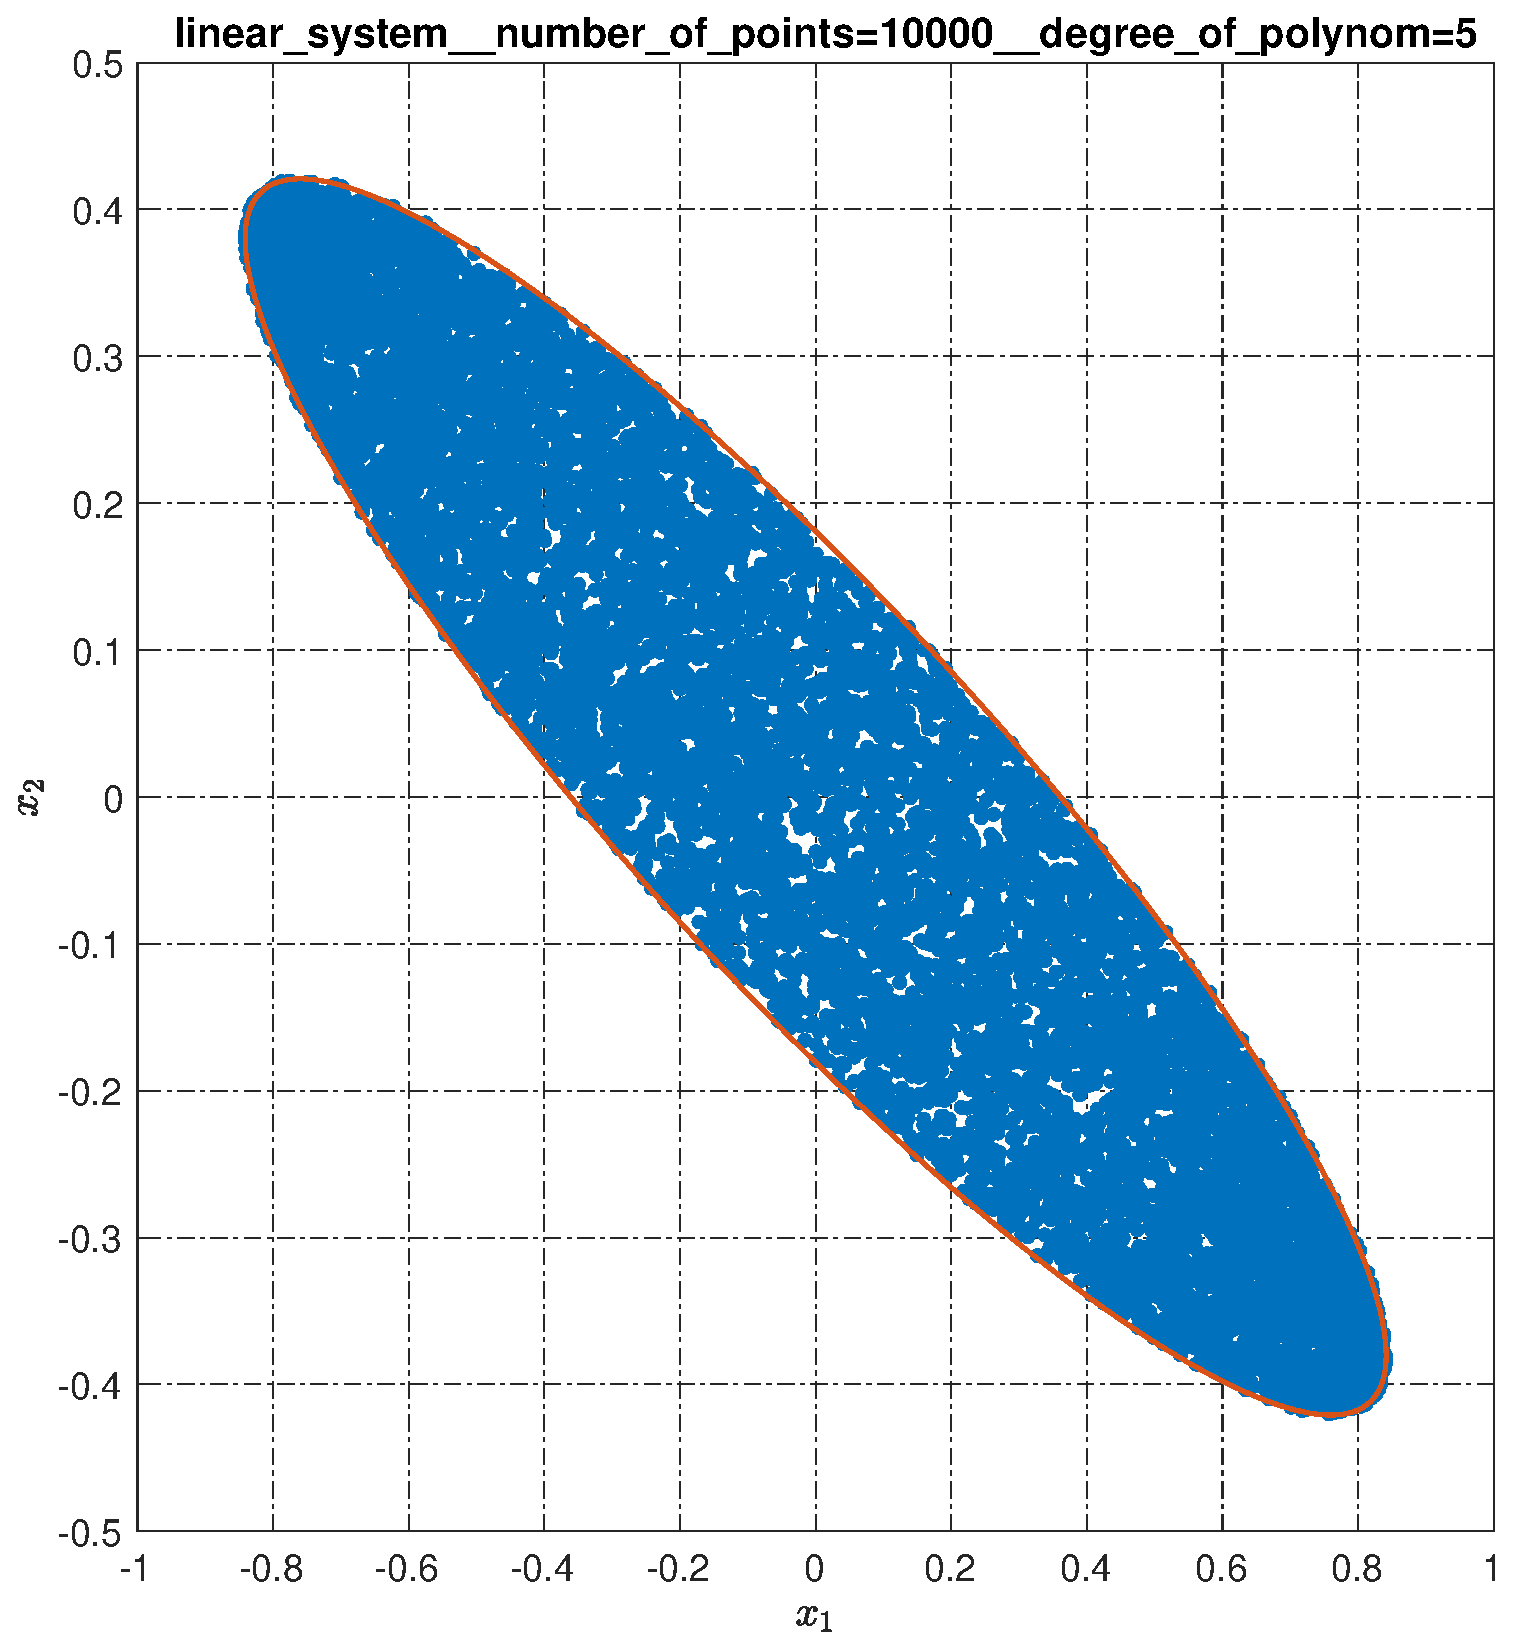
\includegraphics[width=\linewidth]{images/linear_system__number_of_points=10000__degree_of_polynom=5.eps}
  		%\input{OsipovI_u=1_x1-x2_0.tex}
%  		\subcaption{$ \overline{G}_{1,2}(\varepsilon) $ системы \eqref{unicycle1};}
%  		\label{fig:u=1_x1-x2}  
  	\end{minipage} 
  	\vfill
  	\hspace{-2.5ex}
  	\begin{minipage}[b]{.49\linewidth} 
  		\small
  		\centering 
  		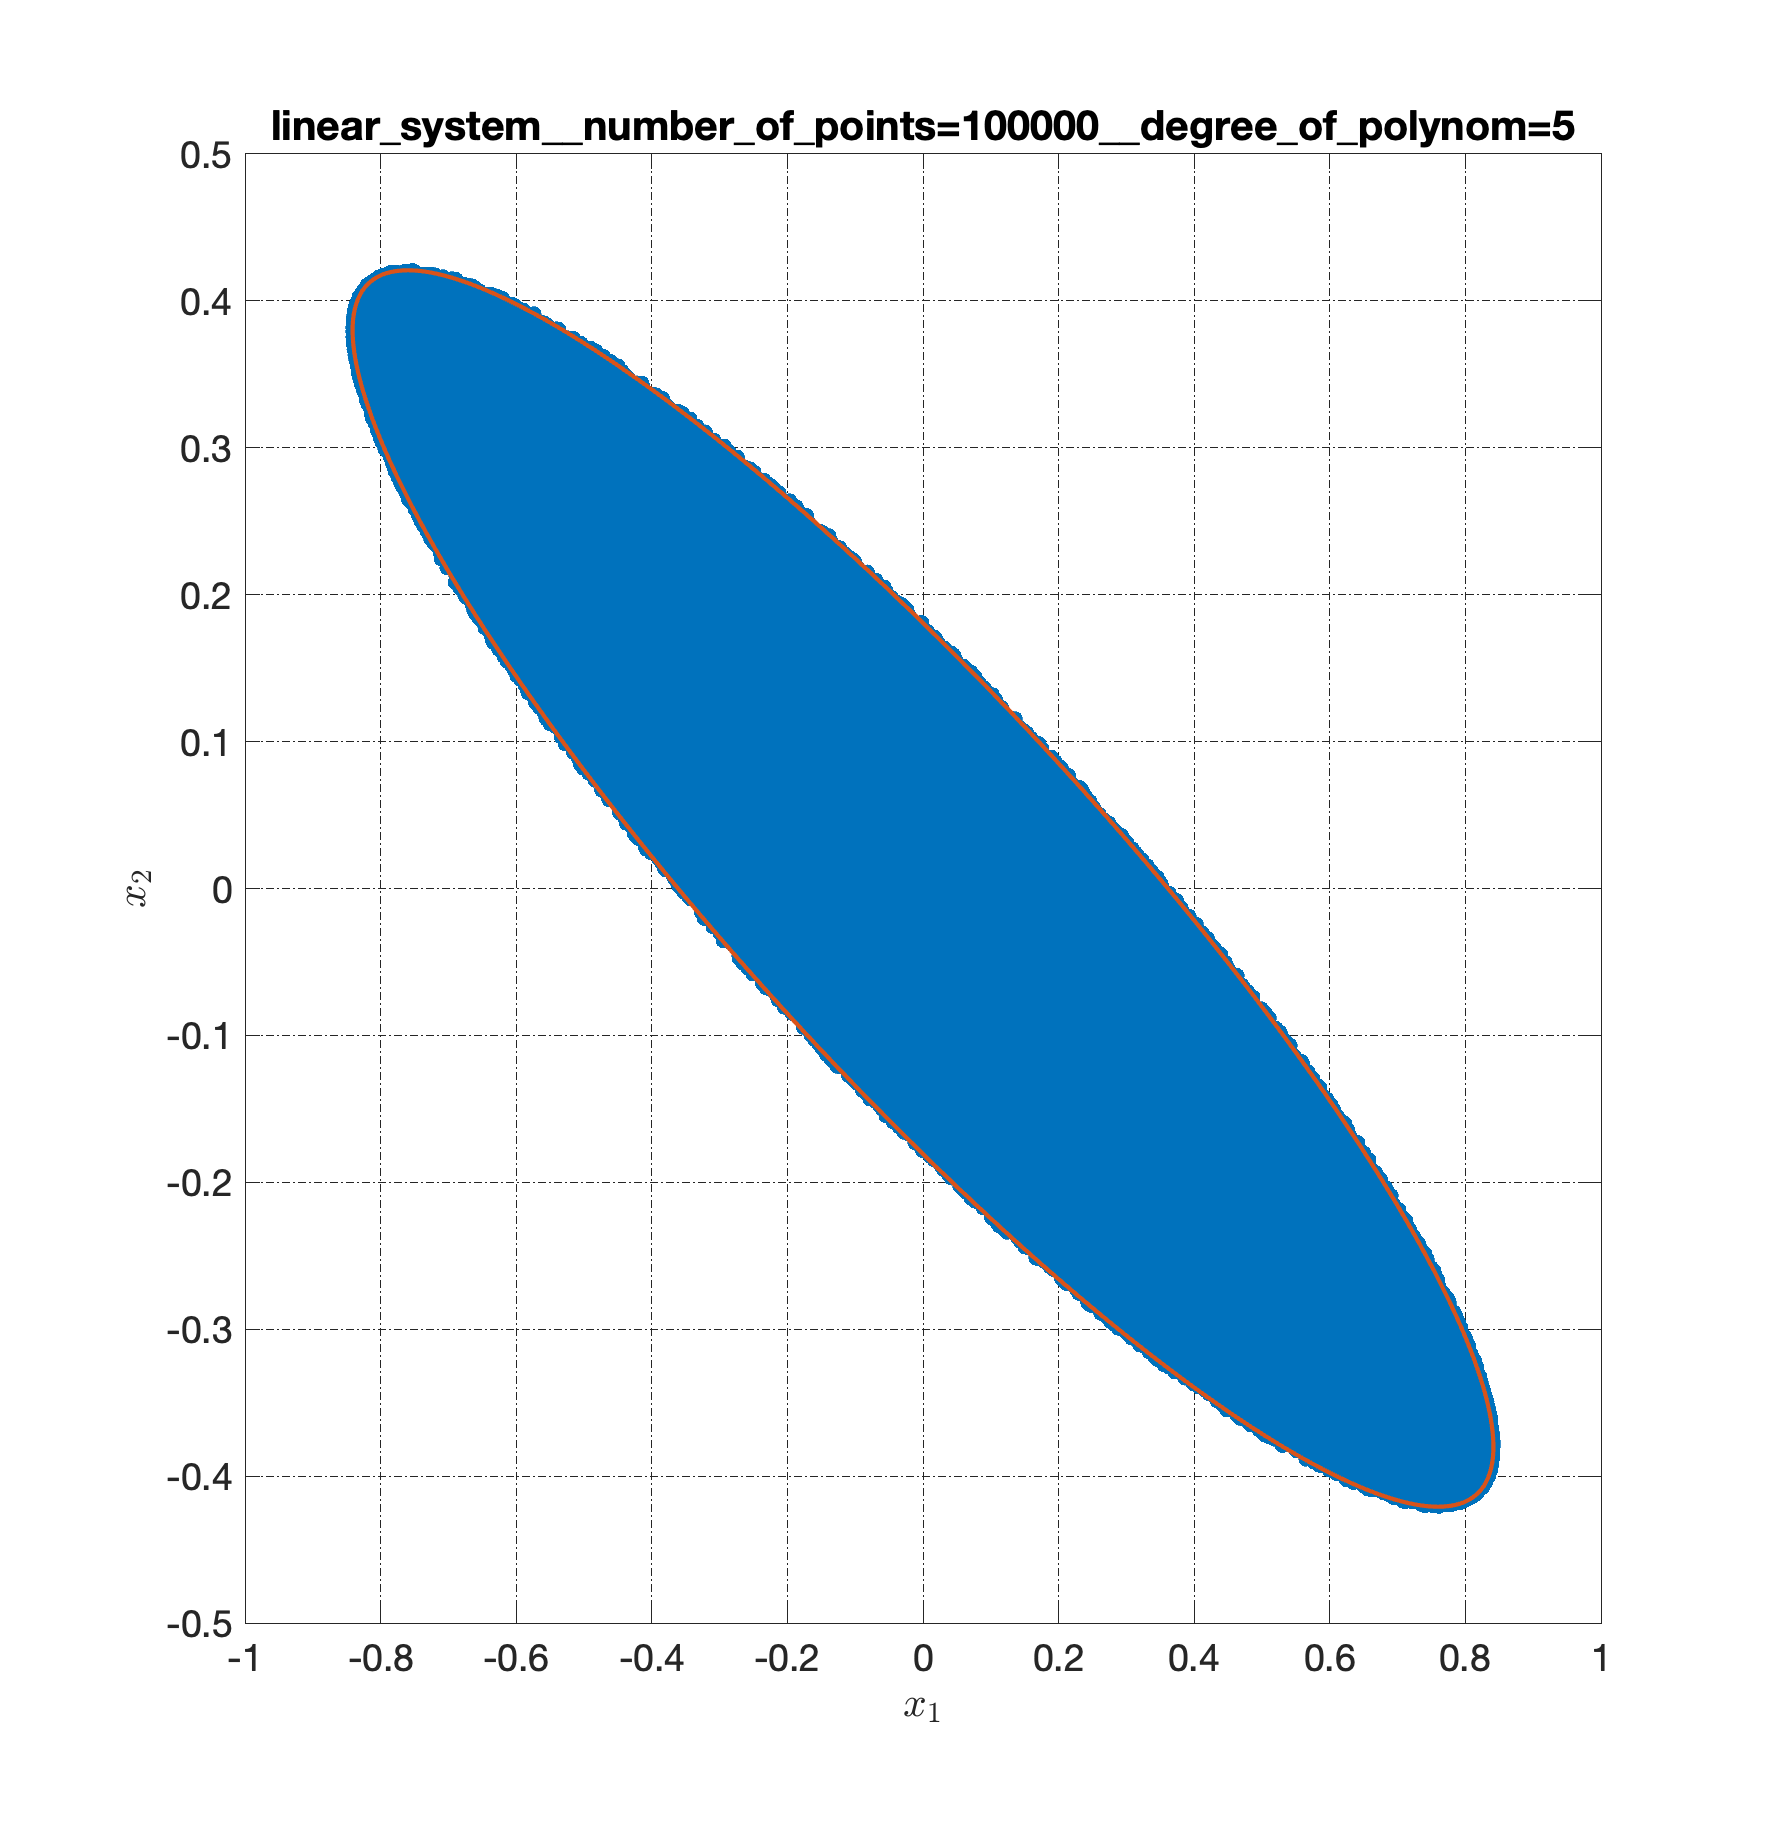
\includegraphics[width=\linewidth]{images/linear_system__number_of_points=100000__degree_of_polynom=5.eps}
  		%% This file was created by matlab2tikz.
%
%The latest updates can be retrieved from
%  http://www.mathworks.com/matlabcentral/fileexchange/22022-matlab2tikz-matlab2tikz
%where you can also make suggestions and rate matlab2tikz.
%
\begin{tikzpicture}
\node at (2.97,2.35) 
{
\includegraphics[width=0.985\linewidth]{OsipovI_u=0_x1-x3_1}};
\pgfkeys{/pgf/number format/.cd,fixed relative,precision=3}
\begin{axis}[%
width=0.761\linewidth,
height=0.6\linewidth,
at={(0\linewidth,0\linewidth)},
scale only axis,
xmin=0.009975,
xmax=0.01,
xlabel style={font=\color{white!15!black}},
ylabel near ticks,
xlabel={$ x_1 $},
ymin=-0.1,
ymax=0.1,
ylabel style={font=\color{white!15!black}},
ylabel={$ x_3 $},
xmajorgrids,
ymajorgrids,
grid style={dashed, opacity=0.7}
]
\end{axis}
\end{tikzpicture}%
%  		\subcaption{$ \overline{G}_{1,3}(\varepsilon) $ системы \eqref{unicycle0};}
%  		\label{fig:u=0_x1-x3} 
  	\end{minipage}
  	\hfill
  	\begin{minipage}[b]{.49\linewidth} 
  		\small
  		\centering
  		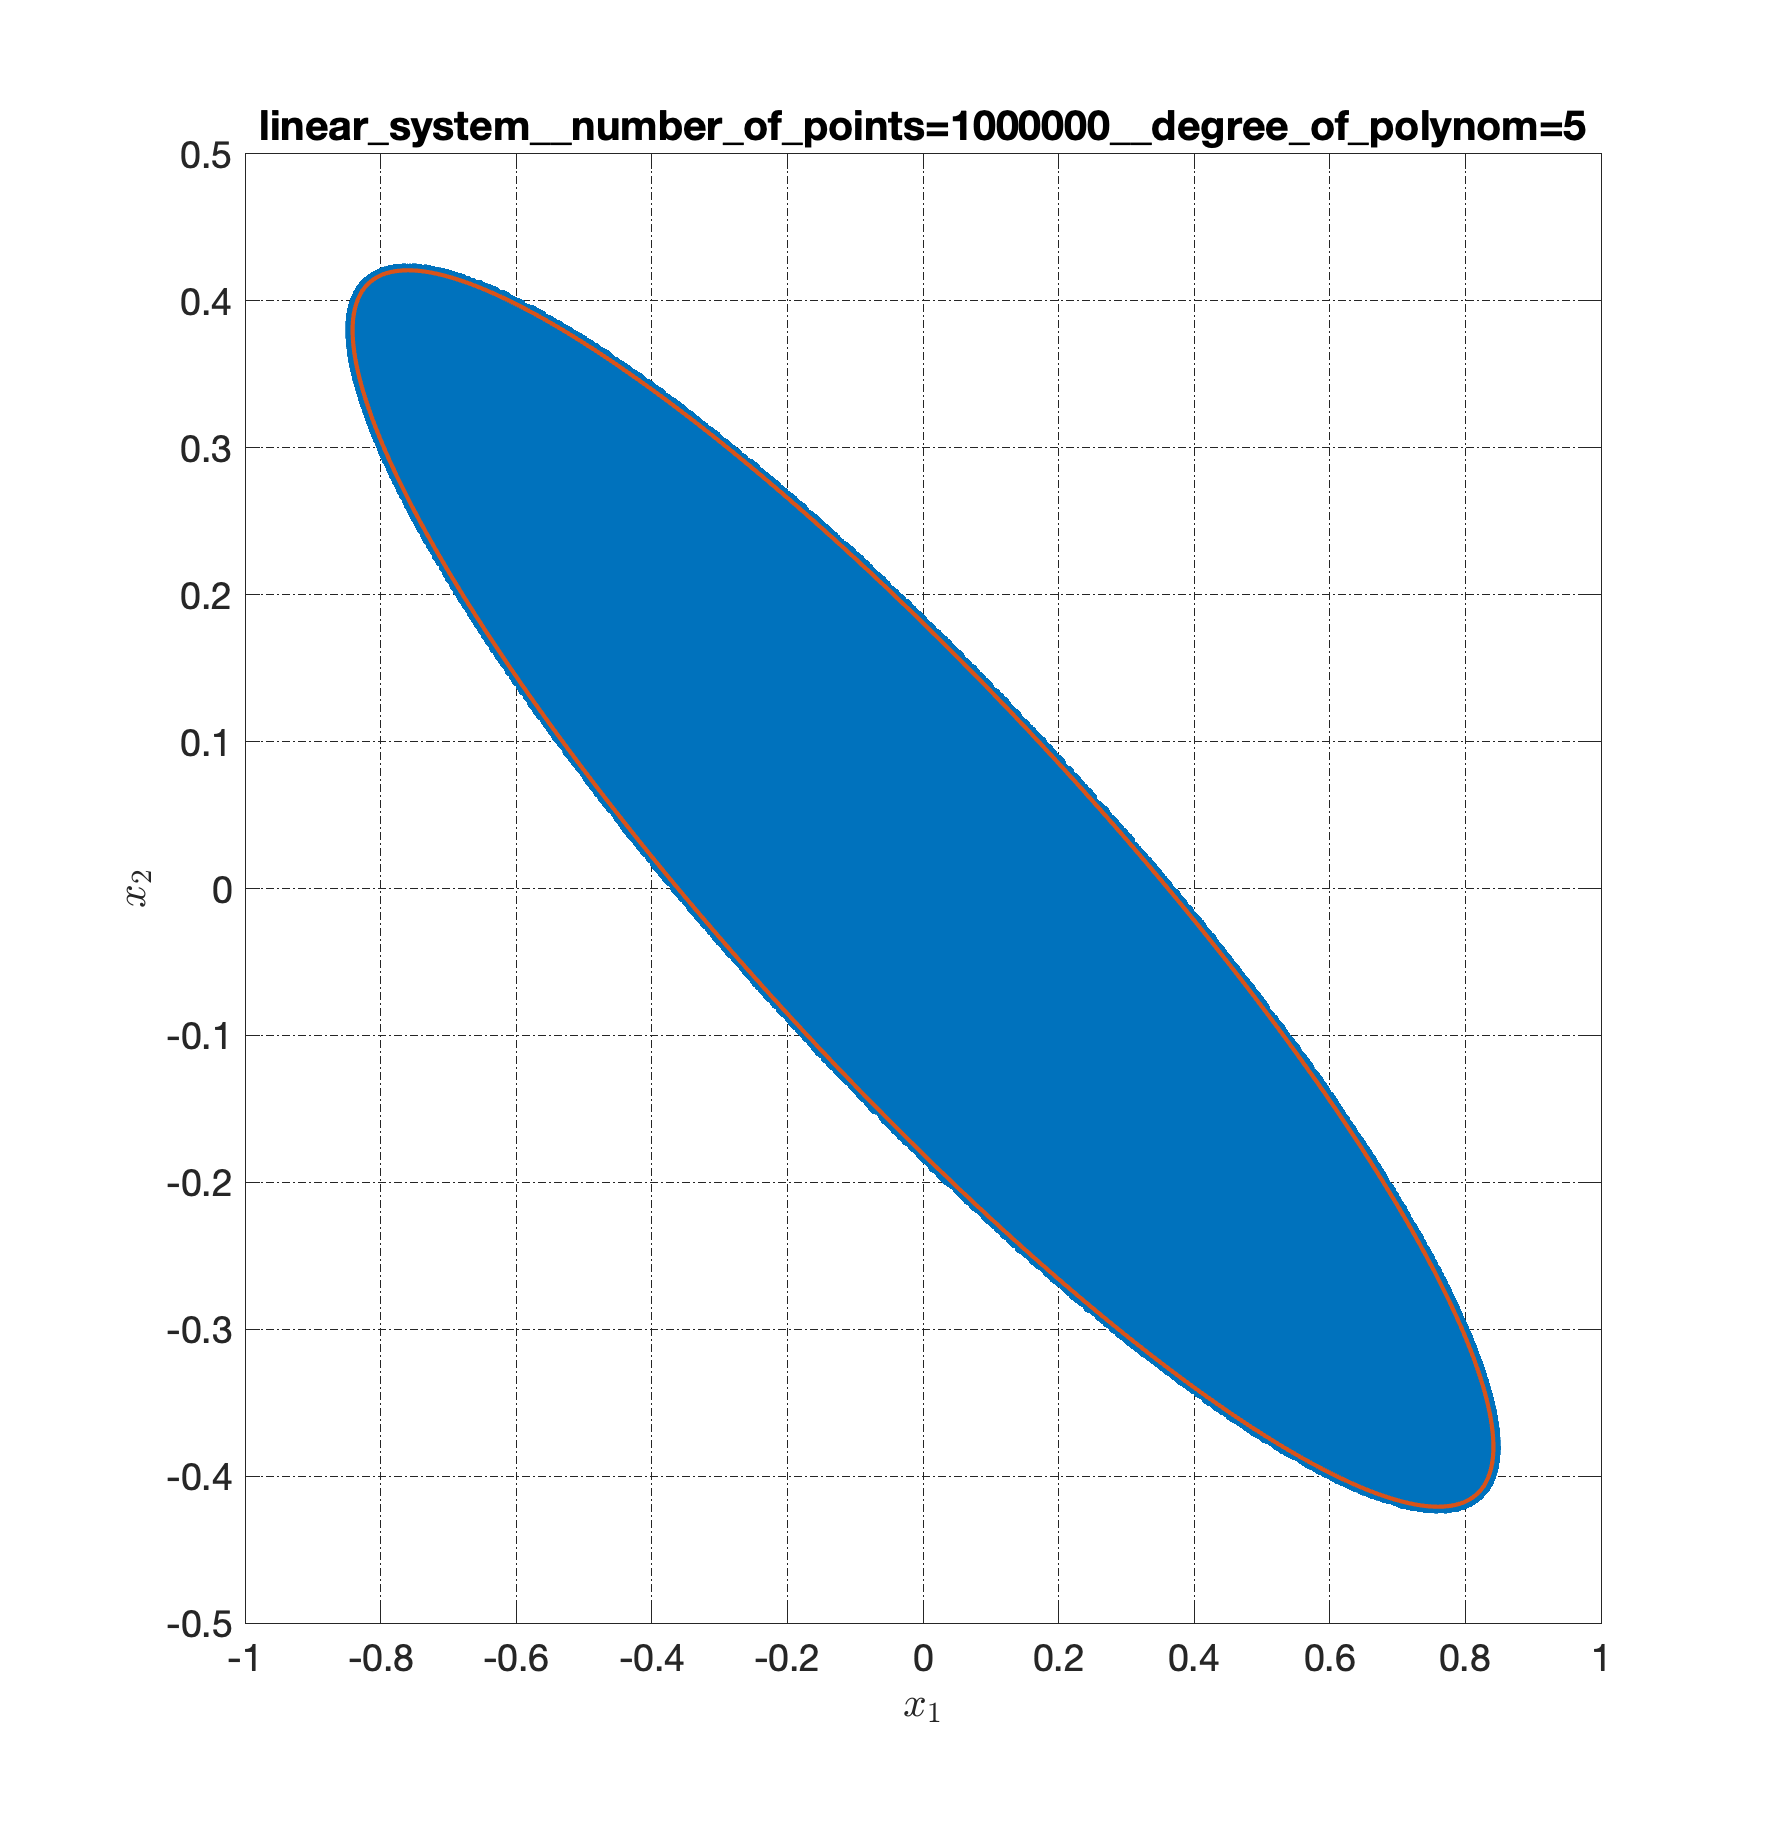
\includegraphics[width=\linewidth]{images/linear_system__number_of_points=1000000__degree_of_polynom=5.eps}
  		%% This file was created by matlab2tikz.
%
%The latest updates can be retrieved from
%  http://www.mathworks.com/matlabcentral/fileexchange/22022-matlab2tikz-matlab2tikz
%where you can also make suggestions and rate matlab2tikz.
%
\begin{tikzpicture}
	
\node at (2.97,2.35) 
{
\includegraphics[width=0.985\linewidth]{OsipovI_u=1_x1-x3_1}};
\pgfkeys{/pgf/number format/relative*={-3}}

\begin{axis}[%
width=0.761\linewidth,
height=0.6\linewidth,
at={(0\linewidth,0\linewidth)},
scale only axis,
xmin=0.009975,
xmax=0.01,
xlabel style={font=\color{white!15!black}},
xlabel={$ x_1 $},
ymin=-0.1,
ymax=0.15,
ylabel style={font=\color{white!15!black}},
ylabel={$ x_3 $},
xmajorgrids,
ymajorgrids,
grid style={dashed, opacity=0.9}
]
\end{axis}
\end{tikzpicture}%
%  		\subcaption{$ \overline{G}_{1,3}(\varepsilon) $ системы \eqref{unicycle1};}
%  		\label{fig:u=1_x1-x3}  
  	\end{minipage} 
%  	\caption{Результаты численного эксперимента для $ \varepsilon = 0.01 $.}\label{fig:RS}
  \end{figure}
  
   \begin{figure}[ht!] 
  	\hspace{-2.5ex}
  	\begin{minipage}[b]{.49\linewidth} 
  		\small
  		\centering 
  		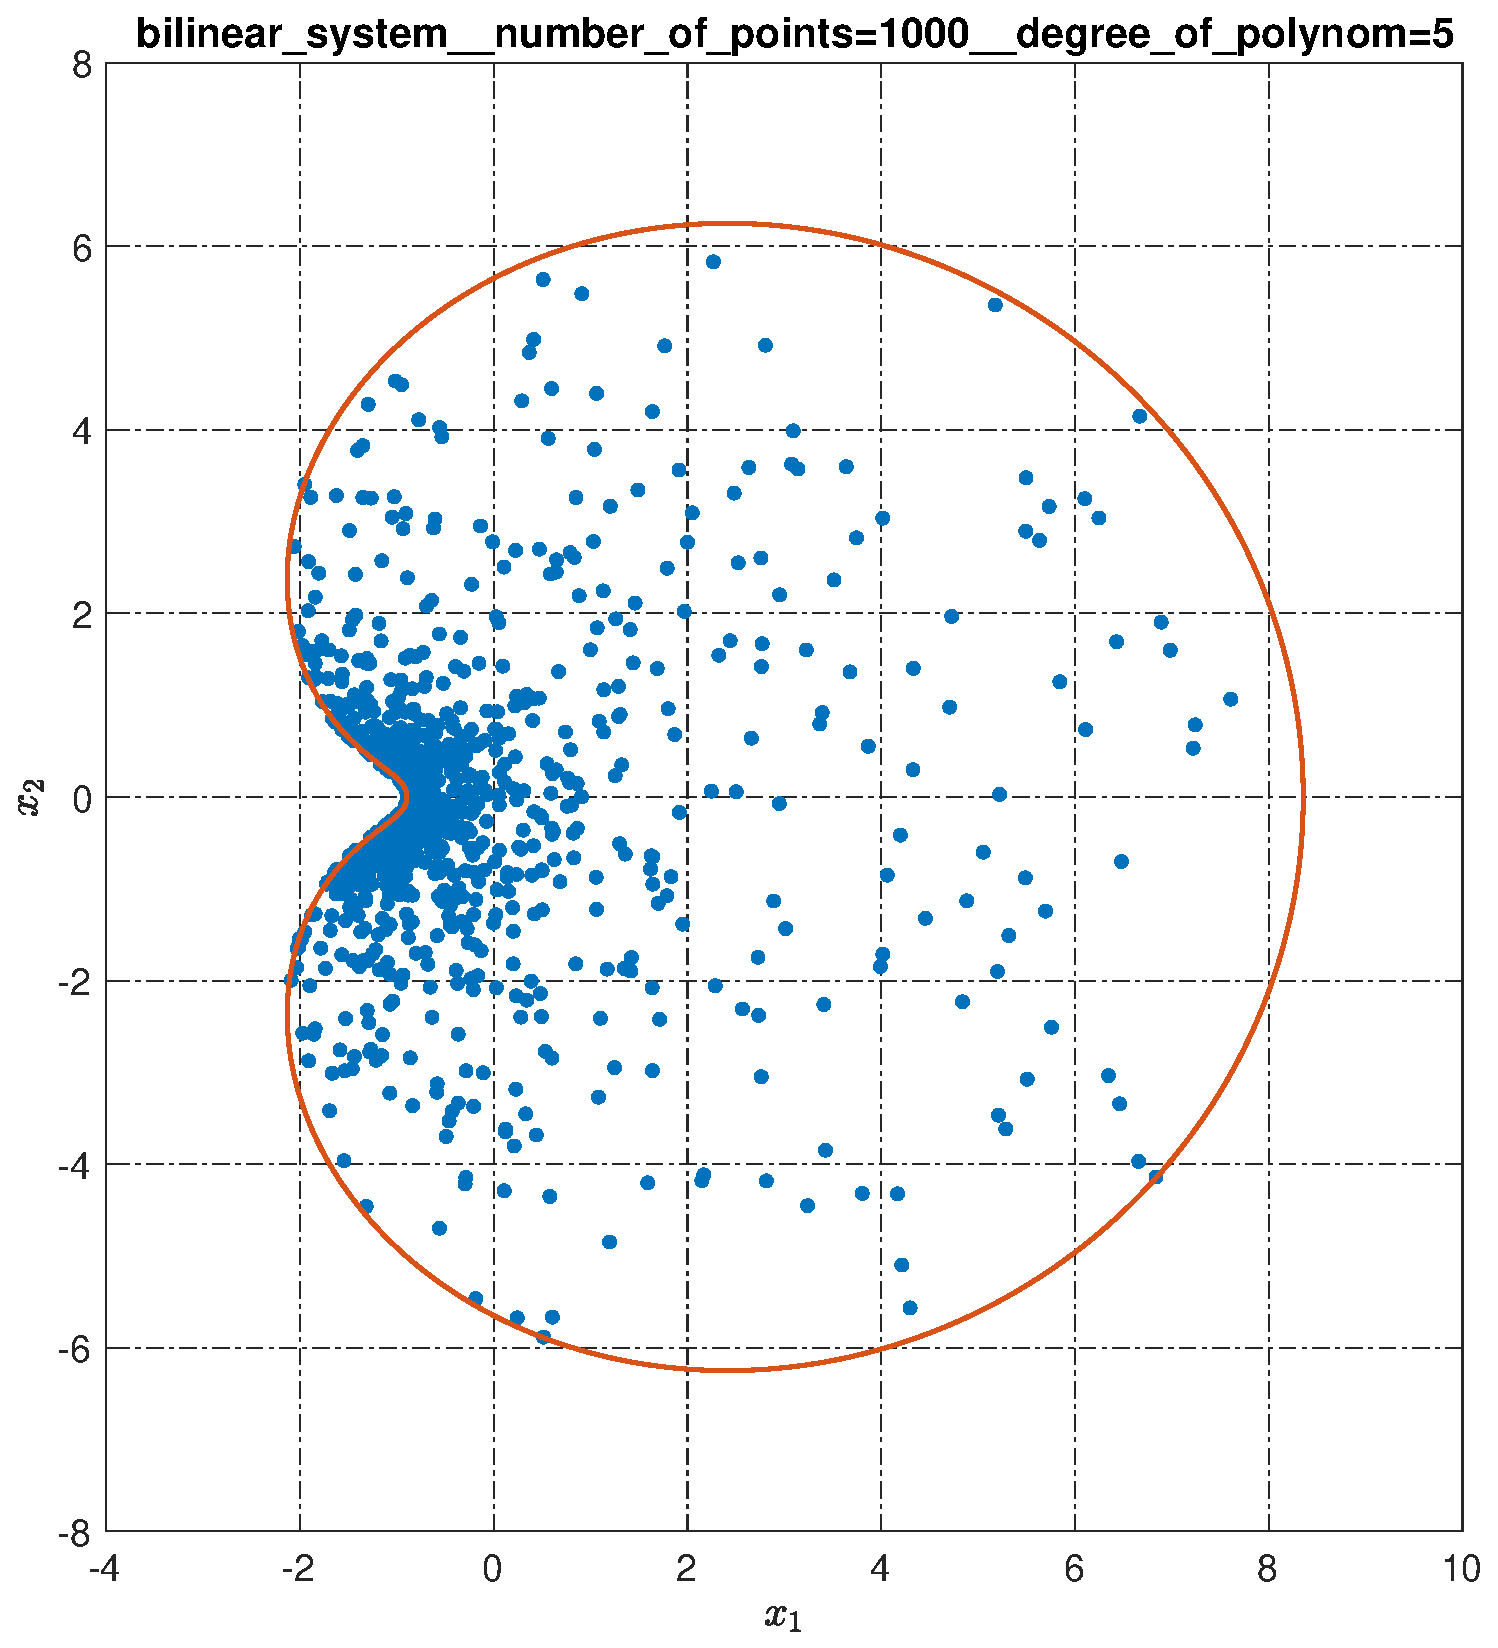
\includegraphics[width=\linewidth]{images/bilinear_system__number_of_points=1000__degree_of_polynom=5.eps}
  		%% This file was created by matlab2tikz.
%
%The latest updates can be retrieved from
%  http://www.mathworks.com/matlabcentral/fileexchange/22022-matlab2tikz-matlab2tikz
%where you can also make suggestions and rate matlab2tikz.
%
\begin{tikzpicture}
\node at (2.97,2.35) 
{
\includegraphics[width=0.985\linewidth]{images/OsipovI_u=0_x1-x2_1.eps}};
\pgfkeys{/pgf/number format/relative*={-3}}
\begin{axis}[%
width=0.761\linewidth,
height=0.6\linewidth,
at={(0\linewidth,0\linewidth)},
scale only axis,
xmin=0.009975,
xmax=0.01,
xlabel style={font=\color{white!15!black}},
xlabel={$ x_1 $},
ymin=-0.0006,
ymax=0.0006,
ylabel style={font=\color{white!15!black}},
ylabel={$ x_2 $},
xmajorgrids,
ymajorgrids,
grid style={dashed, opacity=0.7}
]
\end{axis}
\end{tikzpicture}%
  		%  		\subcaption{$ \overline{G}_{1,2}(\varepsilon) $ системы \eqref{unicycle0};}
  		%  		\label{fig:u=0_x1-x2} 
  	\end{minipage}
  	\hfill
  	\begin{minipage}[b]{.49\linewidth} 
  		\small
  		\centering
  		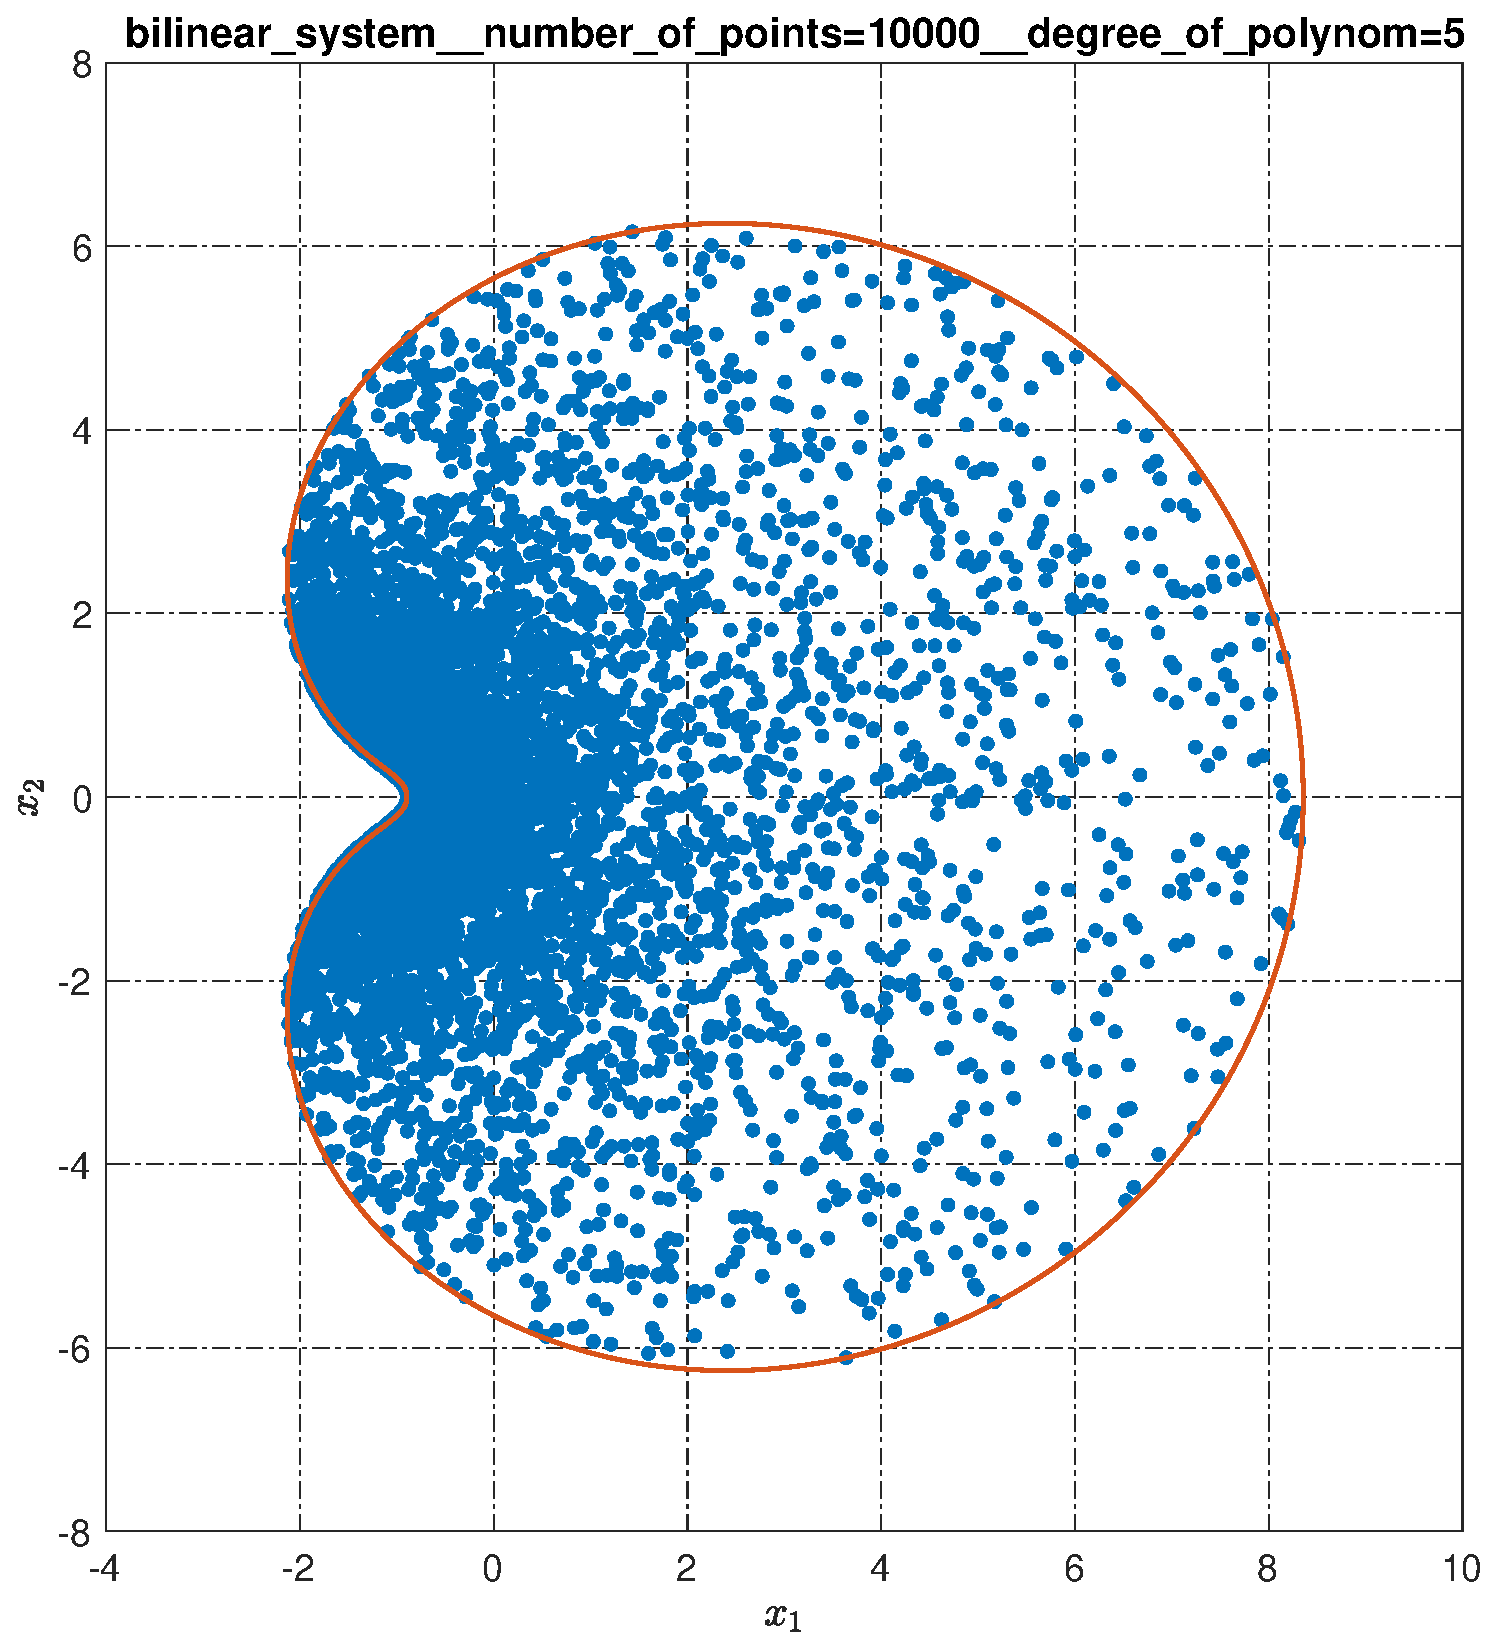
\includegraphics[width=\linewidth]{images/bilinear_system__number_of_points=10000__degree_of_polynom=5.eps}
  		%\input{OsipovI_u=1_x1-x2_0.tex}
  		%  		\subcaption{$ \overline{G}_{1,2}(\varepsilon) $ системы \eqref{unicycle1};}
  		%  		\label{fig:u=1_x1-x2}  
  	\end{minipage} 
  	\vfill
  	\hspace{-2.5ex}
  	\begin{minipage}[b]{.49\linewidth} 
  		\small
  		\centering 
  		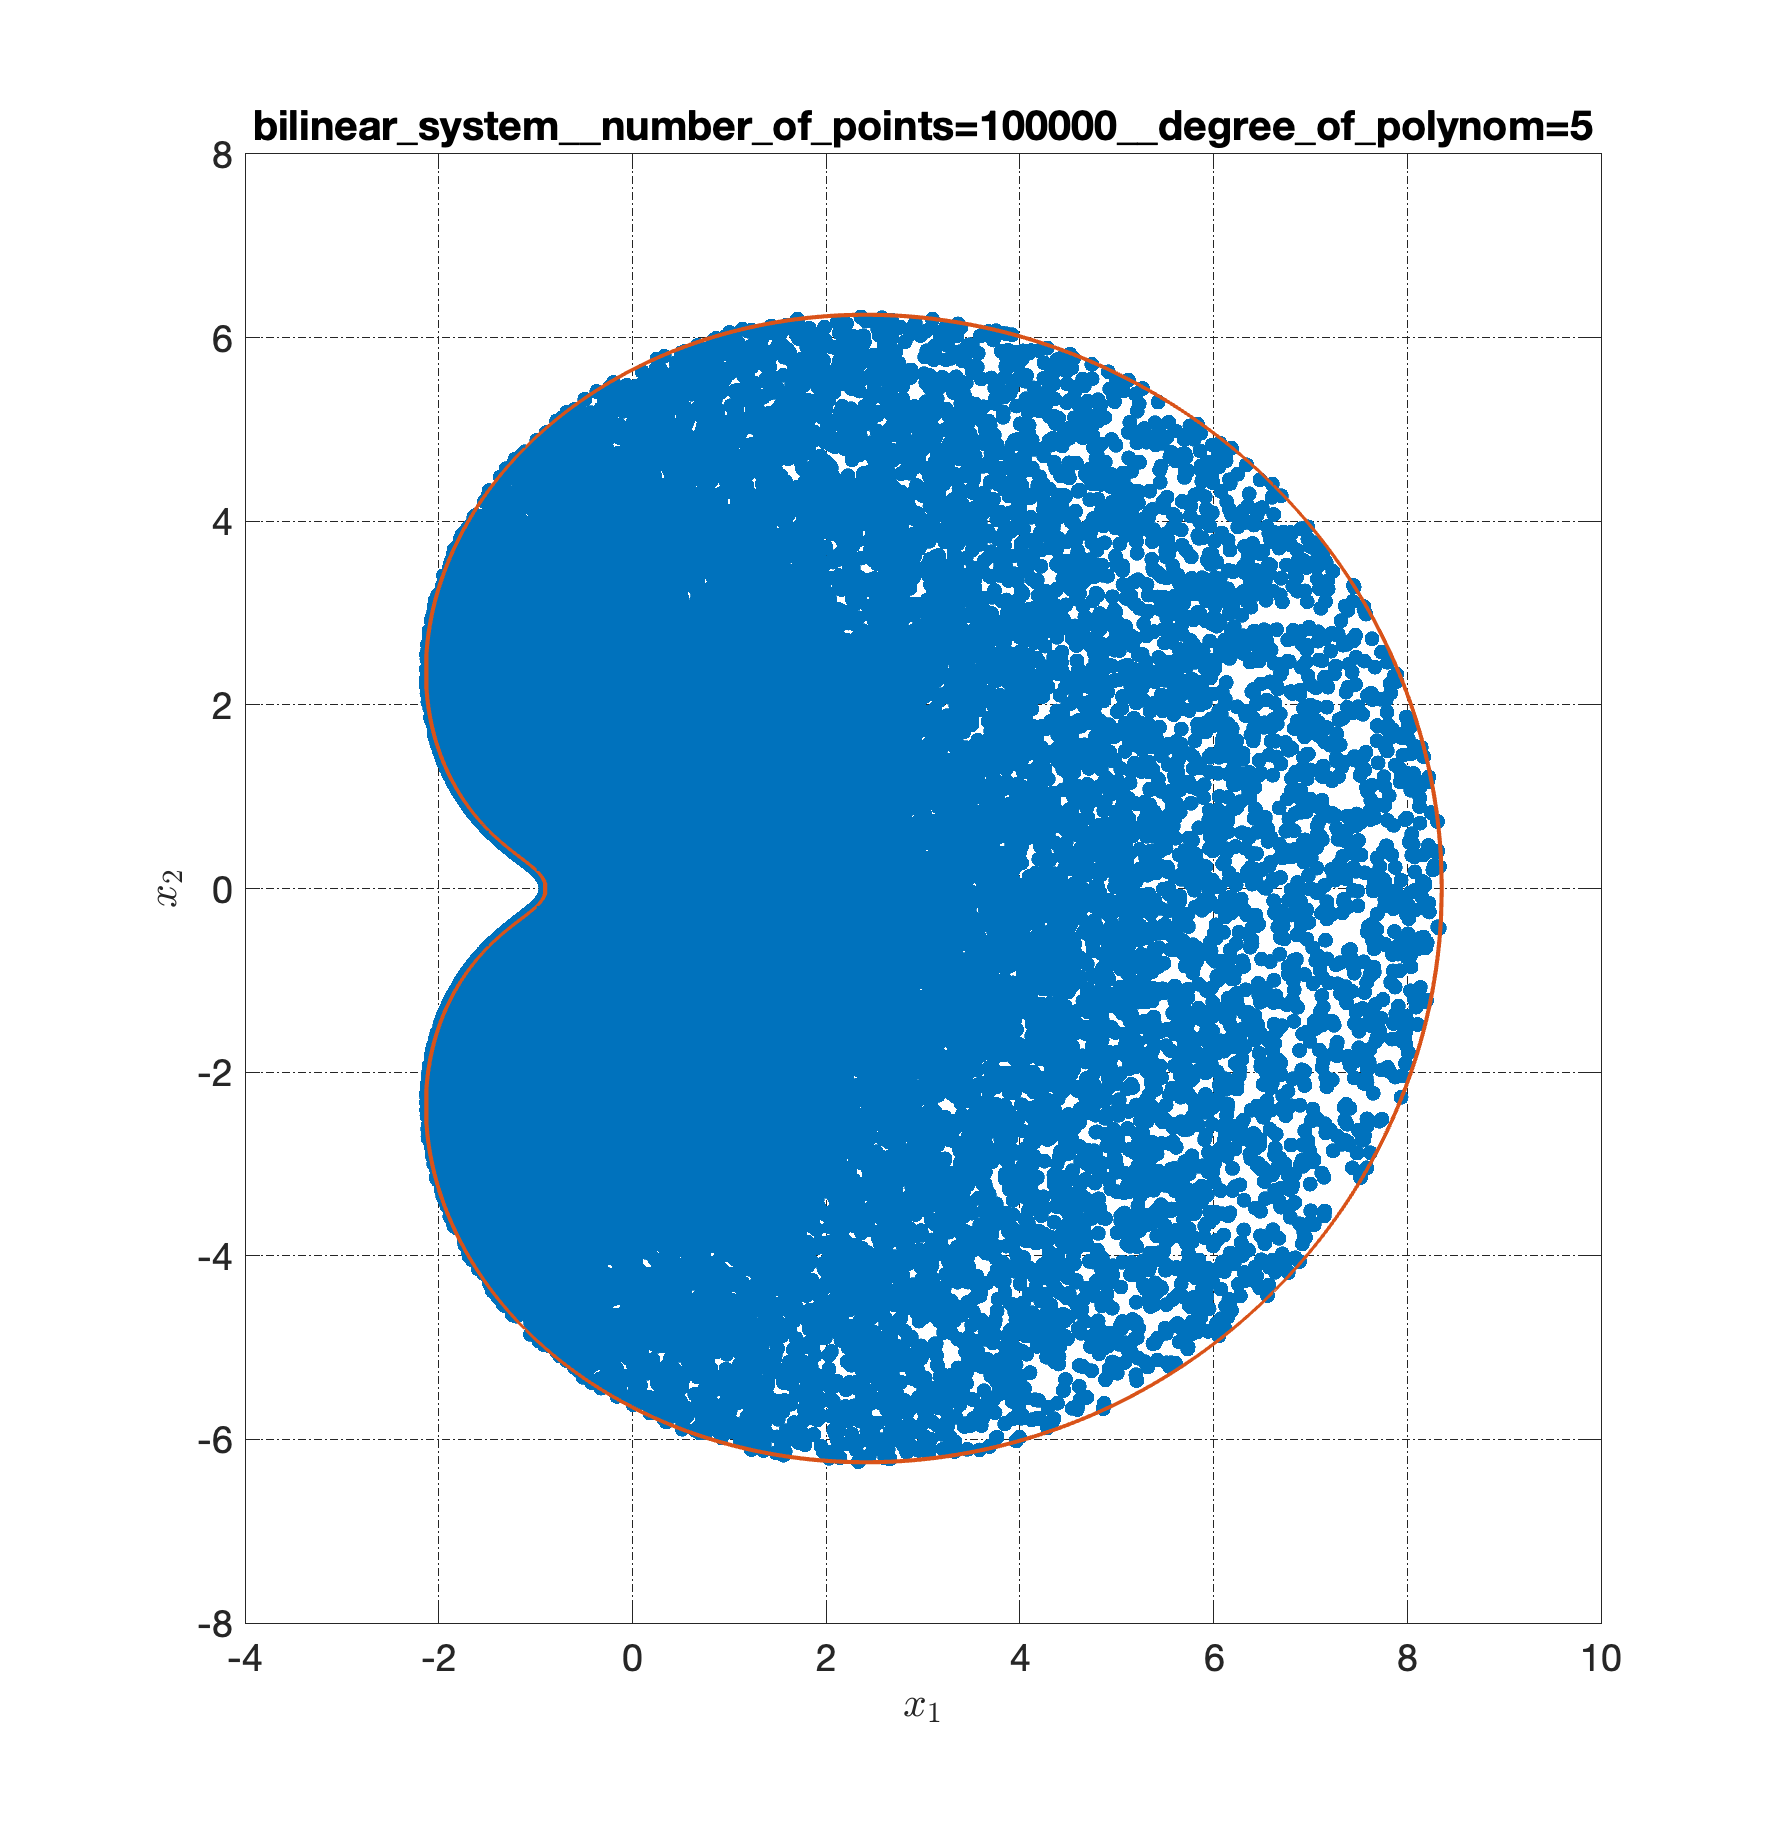
\includegraphics[width=\linewidth]{images/bilinear_system__number_of_points=100000__degree_of_polynom=5.eps}
  		%% This file was created by matlab2tikz.
%
%The latest updates can be retrieved from
%  http://www.mathworks.com/matlabcentral/fileexchange/22022-matlab2tikz-matlab2tikz
%where you can also make suggestions and rate matlab2tikz.
%
\begin{tikzpicture}
\node at (2.97,2.35) 
{
\includegraphics[width=0.985\linewidth]{OsipovI_u=0_x1-x3_1}};
\pgfkeys{/pgf/number format/.cd,fixed relative,precision=3}
\begin{axis}[%
width=0.761\linewidth,
height=0.6\linewidth,
at={(0\linewidth,0\linewidth)},
scale only axis,
xmin=0.009975,
xmax=0.01,
xlabel style={font=\color{white!15!black}},
ylabel near ticks,
xlabel={$ x_1 $},
ymin=-0.1,
ymax=0.1,
ylabel style={font=\color{white!15!black}},
ylabel={$ x_3 $},
xmajorgrids,
ymajorgrids,
grid style={dashed, opacity=0.7}
]
\end{axis}
\end{tikzpicture}%
  		%  		\subcaption{$ \overline{G}_{1,3}(\varepsilon) $ системы \eqref{unicycle0};}
  		%  		\label{fig:u=0_x1-x3} 
  	\end{minipage}
  	\hfill
  	\begin{minipage}[b]{.49\linewidth} 
  		\small
  		\centering
  		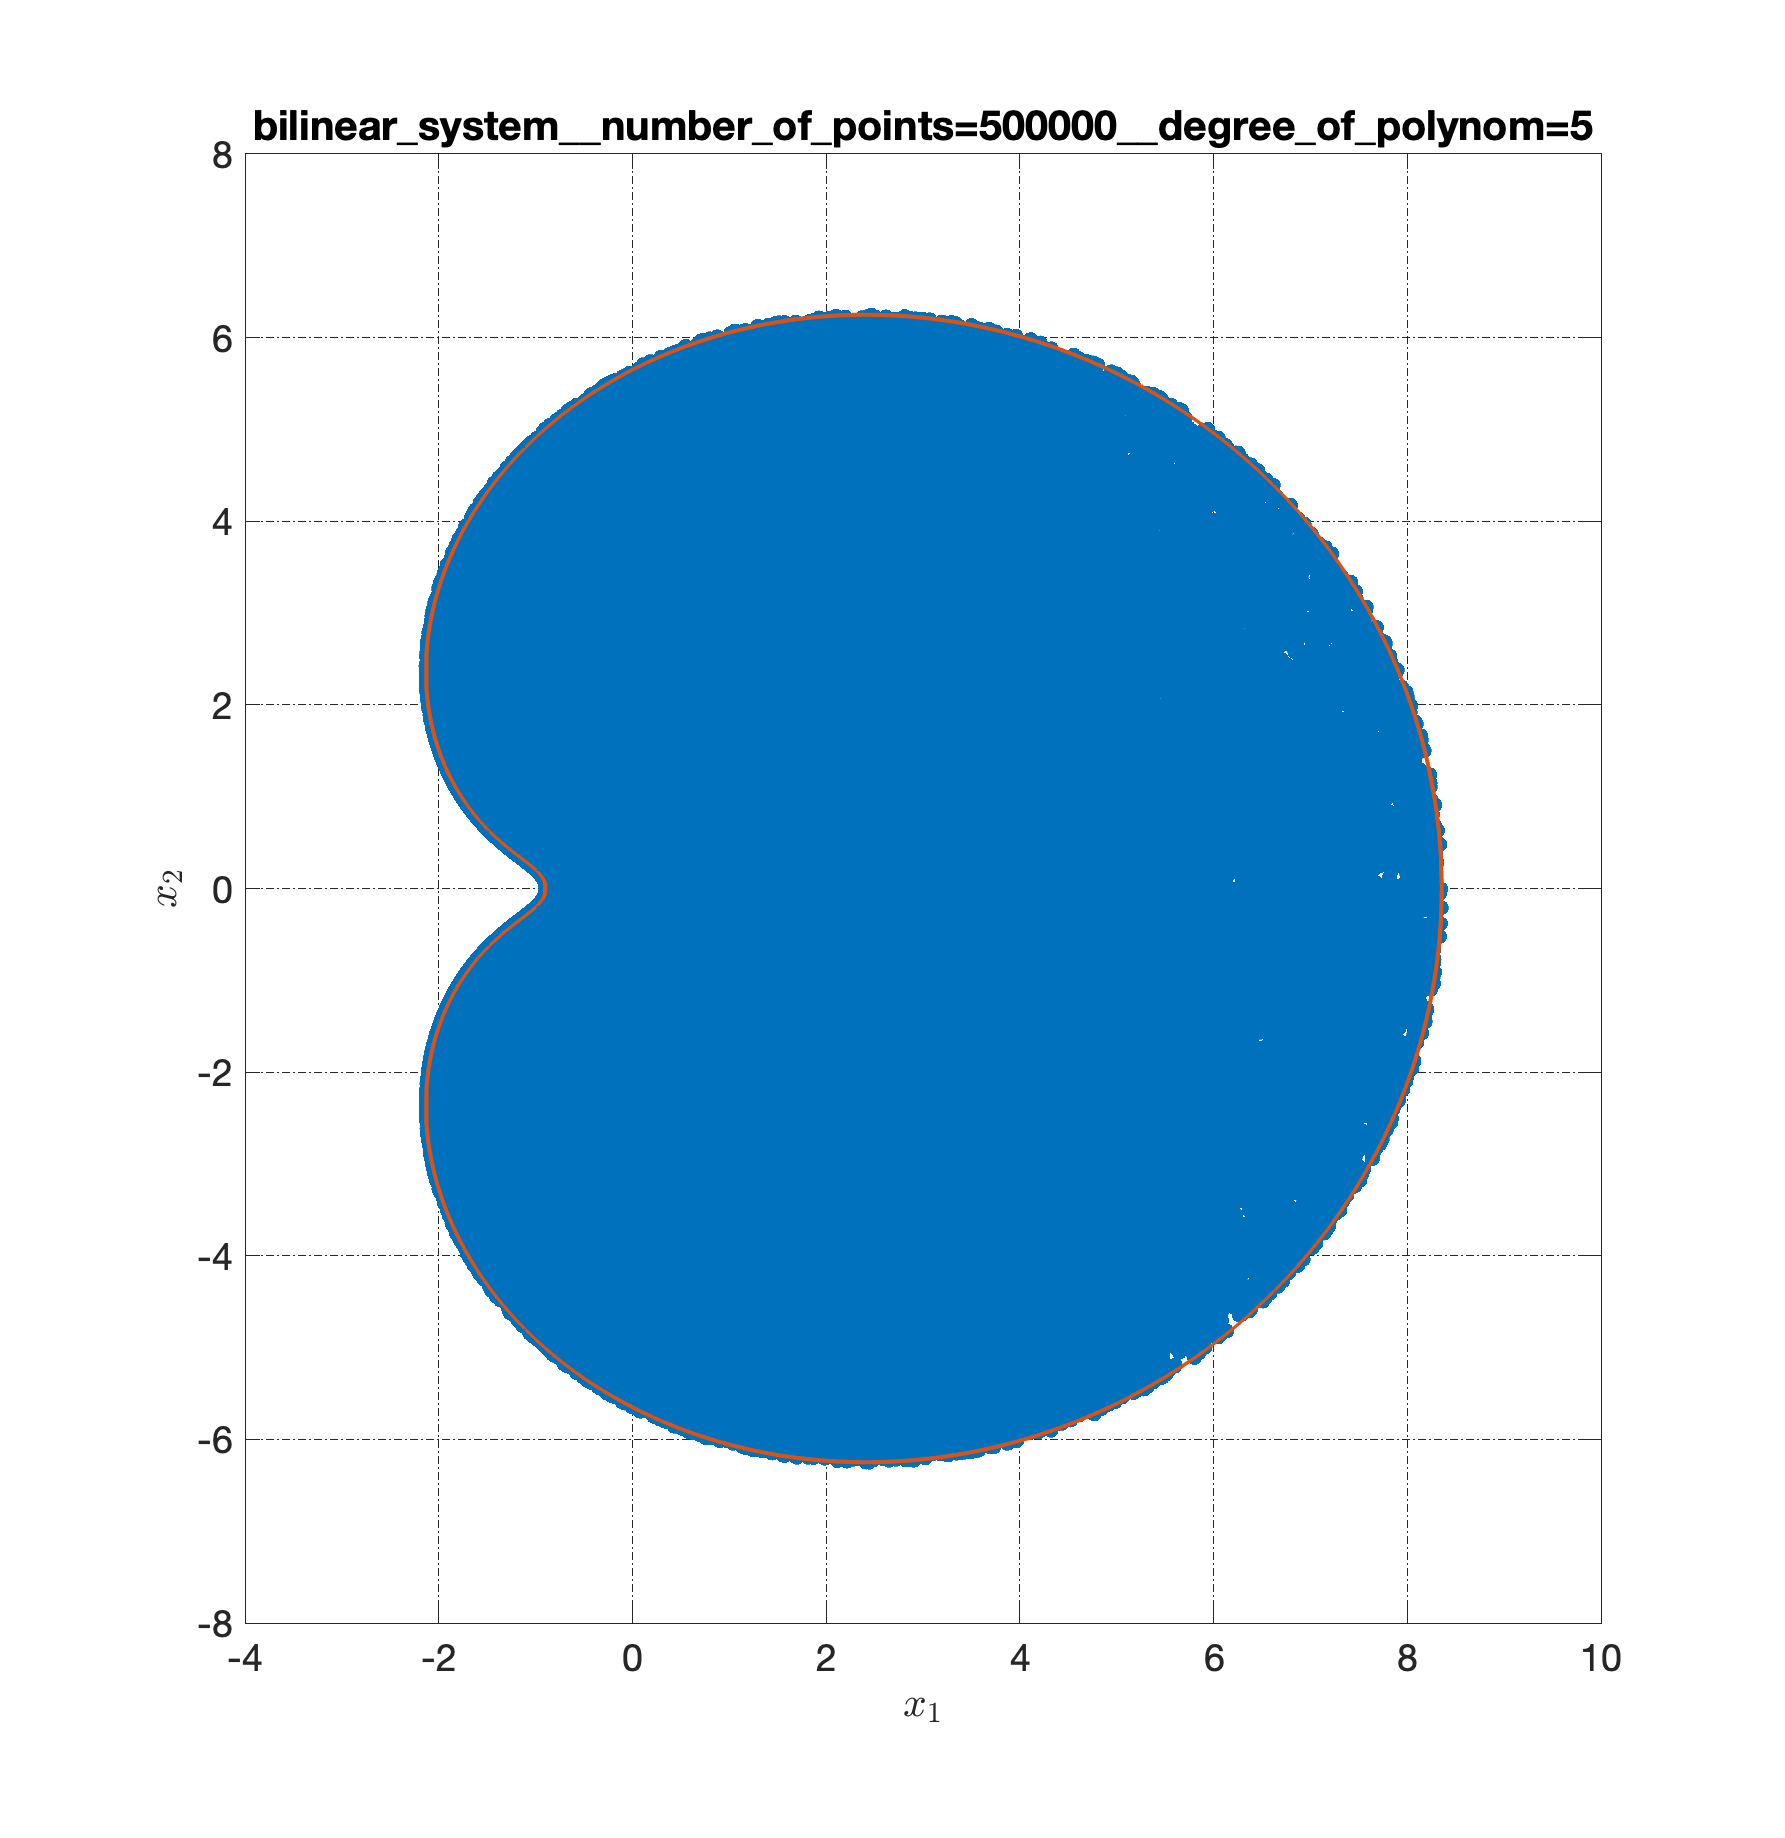
\includegraphics[width=\linewidth]{images/bilinear_system__number_of_points=500000__degree_of_polynom=5.eps}
  		%% This file was created by matlab2tikz.
%
%The latest updates can be retrieved from
%  http://www.mathworks.com/matlabcentral/fileexchange/22022-matlab2tikz-matlab2tikz
%where you can also make suggestions and rate matlab2tikz.
%
\begin{tikzpicture}
	
\node at (2.97,2.35) 
{
\includegraphics[width=0.985\linewidth]{OsipovI_u=1_x1-x3_1}};
\pgfkeys{/pgf/number format/relative*={-3}}

\begin{axis}[%
width=0.761\linewidth,
height=0.6\linewidth,
at={(0\linewidth,0\linewidth)},
scale only axis,
xmin=0.009975,
xmax=0.01,
xlabel style={font=\color{white!15!black}},
xlabel={$ x_1 $},
ymin=-0.1,
ymax=0.15,
ylabel style={font=\color{white!15!black}},
ylabel={$ x_3 $},
xmajorgrids,
ymajorgrids,
grid style={dashed, opacity=0.9}
]
\end{axis}
\end{tikzpicture}%
  		%  		\subcaption{$ \overline{G}_{1,3}(\varepsilon) $ системы \eqref{unicycle1};}
  		%  		\label{fig:u=1_x1-x3}  
  	\end{minipage} 
  	%  	\caption{Результаты численного эксперимента для $ \varepsilon = 0.01 $.}\label{fig:RS}
  \end{figure}
  \subsection{Влияние выбора коэффициентов }
  \subsection{Особенность линейных управлений}
  \subsection{Другие примеры}
  
\end{document}